\documentclass{article}

% 导入宏包
\usepackage{fancyhdr}
\usepackage{ctex}
\usepackage{listings}
\usepackage{graphicx}
\usepackage[a4paper, body={18cm,22cm}]{geometry}
\usepackage{amsmath,amssymb,amstext,wasysym,enumerate,graphicx}
\usepackage{float,abstract,booktabs,indentfirst,amsmath}
\usepackage{array}
\usepackage{multirow}
\usepackage{url}
\usepackage{diagbox}
\usepackage{enumitem}
\usepackage{xcolor}
\usepackage{makecell}
\usepackage{tikz}
\usetikzlibrary{positioning, arrows.meta}

% 设置段落
\renewcommand\arraystretch{1.4}
\setlength{\parindent}{2em}
\setCJKmonofont{黑体}

% 配置代码显示
\lstset{
	xleftmargin = 3em,
	xrightmargin = 3em,
	aboveskip = 1em,
	backgroundcolor = \color{white},
	basicstyle = \small\ttfamily,
	rulesepcolor = \color{gray},
	breaklines = true,
	numbers = left,
	numberstyle = \small,
	numbersep = -14pt,
	keywordstyle = \color{purple}\bfseries,
	commentstyle = \color{green!60!black}, % 修改注释颜色
	stringstyle = \color{red!60!green!90!blue!90},
	morekeywords = {ASSERT, int64_t, uint32_t},
	moreemph = {ASSERT, NULL},
	emphstyle = \color{red}\bfseries,
	moreemph = [2]{int64\_t, uint32\_t, tid\_t, uint8\_t, int16\_t, uint16\_t, int32\_t, size\_t, bool},
	emphstyle = [2]\color{purple}\bfseries,
	frame = shadowbox,
	showspaces = false,
	columns = fixed
	morecomment = [l][\color{green!60!black}]{+}, % 设置以+开头的代码行为绿色
}

%--------------------页眉--------------------%

\pagestyle{fancy}
\fancyhead[L]{}
\fancyhead[R]{}
\fancyhead[C]{华东师范大学软件工程学院实验报告}
\fancyfoot[C]{-\thepage-}
\renewcommand{\headrulewidth}{1.5pt}

%--------------------标题--------------------%

\begin{document}
	\begin{center}
		{\Large{\textbf{\heiti 华东师范大学软件工程学院实验报告}}}
		\begin{table}[htb]
			\flushleft
			\begin{tabular}{p{0.4\linewidth}p{0.27\linewidth}p{0.28\linewidth}}\\
				\textbf{实验课程}:计算机网络实践  & \textbf{年级}:2023级       & \textbf{实验成绩}:  \\
				\textbf{实验名称}:ARP & \textbf{姓名}:顾翌炜         &                 \\
				\textbf{实验编号}:Lab-4     & \textbf{学号}:10235101527 & \textbf{实验日期}:2024/12/13  \\
				\textbf{指导教师}:王廷     & \textbf{组号}:01            & \textbf{实验时间}:2024/12/13  \\ 
			\end{tabular}
		\end{table}
	\end{center}
	\rule{\textwidth}{2pt}
	
	%--------------------正文--------------------%
	\section{实验目的}
	
	\begin{enumerate}[noitemsep, label={{\arabic*})}]
		\item 通过Wireshark获取ARP消息
		\item 掌握ARP数据包结构
		\item 掌握ARP数据包各字段的含义
		\item 了解ARP协议适用领域
	\end{enumerate}
	
	\section{实验内容与实验步骤}
	
	\subsection{实验内容}
	
	\subsubsection{捕获数据}
	
	启动 \texttt{Wireshark},通过菜单栏中的“捕获 $\to$ 选项”进行设置,选择当前连接的以太网接口,并将捕获过滤器设为\texttt{arp},以捕获\texttt{arp}数据包。
	
	接着,在命令提示符中运行\texttt{ipconfig -all}命令,以便获取本机的\texttt{IP}地址和\texttt{MAC}地址。
	
	随后,在 \texttt{Wireshark} 的显示过滤器中输入\texttt{eth.addr==<yourMAC>}
	(请将\texttt{<yourMAC>}替换为本机的实际\texttt{MAC}地址)。
	
	然后,以管理员权限打开命令提示符,执行\texttt{arp -d}命令以清空本机的\texttt{ARP}缓存。
	
	最后,重新打开 \texttt{Wireshark},并停止捕获。
	
	\subsubsection{回答问题}
	
	\begin{enumerate}[noitemsep]
		
		\item Hand in your drawing of the ARP exchange.
		\item What opcode is used to indicate a request? What about a reply?
		\item How large is the ARP header for a request? What about for a reply?
		\item What value is carried on a request for the unknown target MAC address?
		\item What Ethernet Type value which indicates that ARP is the higher layer protocol?
		\item Is the ARP reply broadcast (like the ARP request) or not?
		
	\end{enumerate}
	
	\subsubsection{问题讨论}
	
	We encourage you to explore ARP on your own once you have completed this lab. One suggestion is to look at other ARP packets that may have been recorded in your trace; we only examined an ARP request by your computer and the ARP reply from the default gateway. 
	
	\begin{enumerate}
		
		\item ARP requests broadcast by other computers. The other computers on the local network are also using ARP. Since requests are broadcast, your computer will receive their requests. 
		\item ARP replies sent by your computer. If another computer happens to ARP for the IP address of your computer, then your computer will send an ARP reply to tell it the answer. 
		\item Gratuitous ARPs in which your computer sends a request or reply about itself. This is helpful when a computer or link comes up to make sure that no-one else is using the same IP address. Gratuitous ARPs have the same sender and target IP address, and they have an Info field in Wireshark that identified them as gratuitous.
		\item Other ARP requests sent by your computer and the corresponding ARP reply. Your computer may need to ARP for other hosts besides the default gateway after you flush its ARP cache. 
		
	\end{enumerate}
	
	\subsection{实验步骤}
	
	\begin{enumerate}[noitemsep, label={{\arabic*})}]
		
		\item 启动 \texttt{Wireshark},在菜单栏的“捕获 $\to$ 选项”中进行设置,选择已连接的以太网接口,将捕获过滤器设置为 \texttt{arp},并将混杂模式关闭,然后开始捕获。
		\item 在命令行中使用 \texttt{ipconfig -all} 命令获取本机的 \texttt{IP} 地址和 \texttt{MAC} 地址。
		\begin{lstlisting}
        C:\User\GHOST> ipconfig -all
		\end{lstlisting}
		\item 返回 \texttt{Wireshark},设置捕获过滤器为 \texttt{eth.addr==<yourMAC>}
		\item 在管理员模式下,使用 \texttt{arp -d} 命令清除本机的 \texttt{ARP} 缓存。
		\begin{lstlisting}
        C:\User\GHOST> arp -d
		\end{lstlisting}
		\item 打开 \texttt{Wireshark},停止捕获。
		\item 分析捕获到的 \texttt{ARP} 数据包,并回答相关问题。
		\item 对捕获的 \texttt{ARP} 数据包进行详细分析,并回答相关问题。
		\item 讨论问题
	\end{enumerate}
	
	\section{实验环境}
	
	\begin{itemize}[noitemsep]
		\item 操作系统:\texttt{Windows 11 家庭中文版 23H2 22631.4460}
		\item 网络适配器:\texttt{Killer(R)Wi-Fi 6E AX1675i 160MHz Wireless Network Adapter(211NGW)}
		\item \texttt{Wireshark}:\texttt{Version 4.4.1}
		\item \texttt{wget}:\texttt{GNU Wget 1.21.4 built on mingw32}
	\end{itemize}
	
	\section{实验过程与分析}
	
	\subsection{捕获数据}
	
	首先,启动 \texttt{Wireshark},通过菜单栏中的“捕获 $\to$ 选项”进行设置,选择已连接的以太网接口,将捕获过滤器设置为 \texttt{arp},并将混杂模式关闭,然后开始捕获。
	
	\begin{figure}[H]
		\centering
		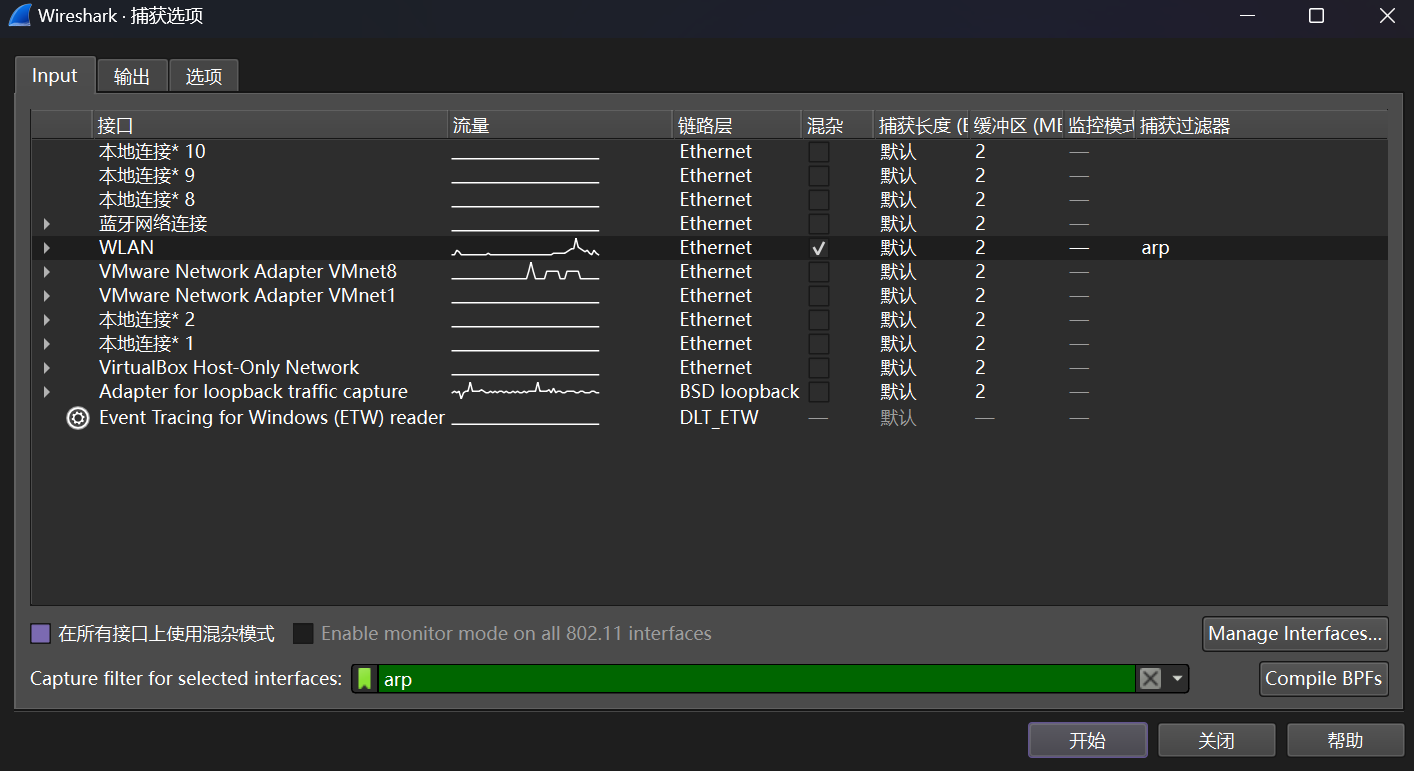
\includegraphics[width=11cm]{images/1.设置捕获.png}
		\caption{设置捕获}
	\end{figure}
	
	然后在命令提示符中使用\texttt{ipconfig -all}命令获取本机的\texttt{IP}地址和\texttt{MAC}地址。
	
	\begin{figure}[H]
		\centering
		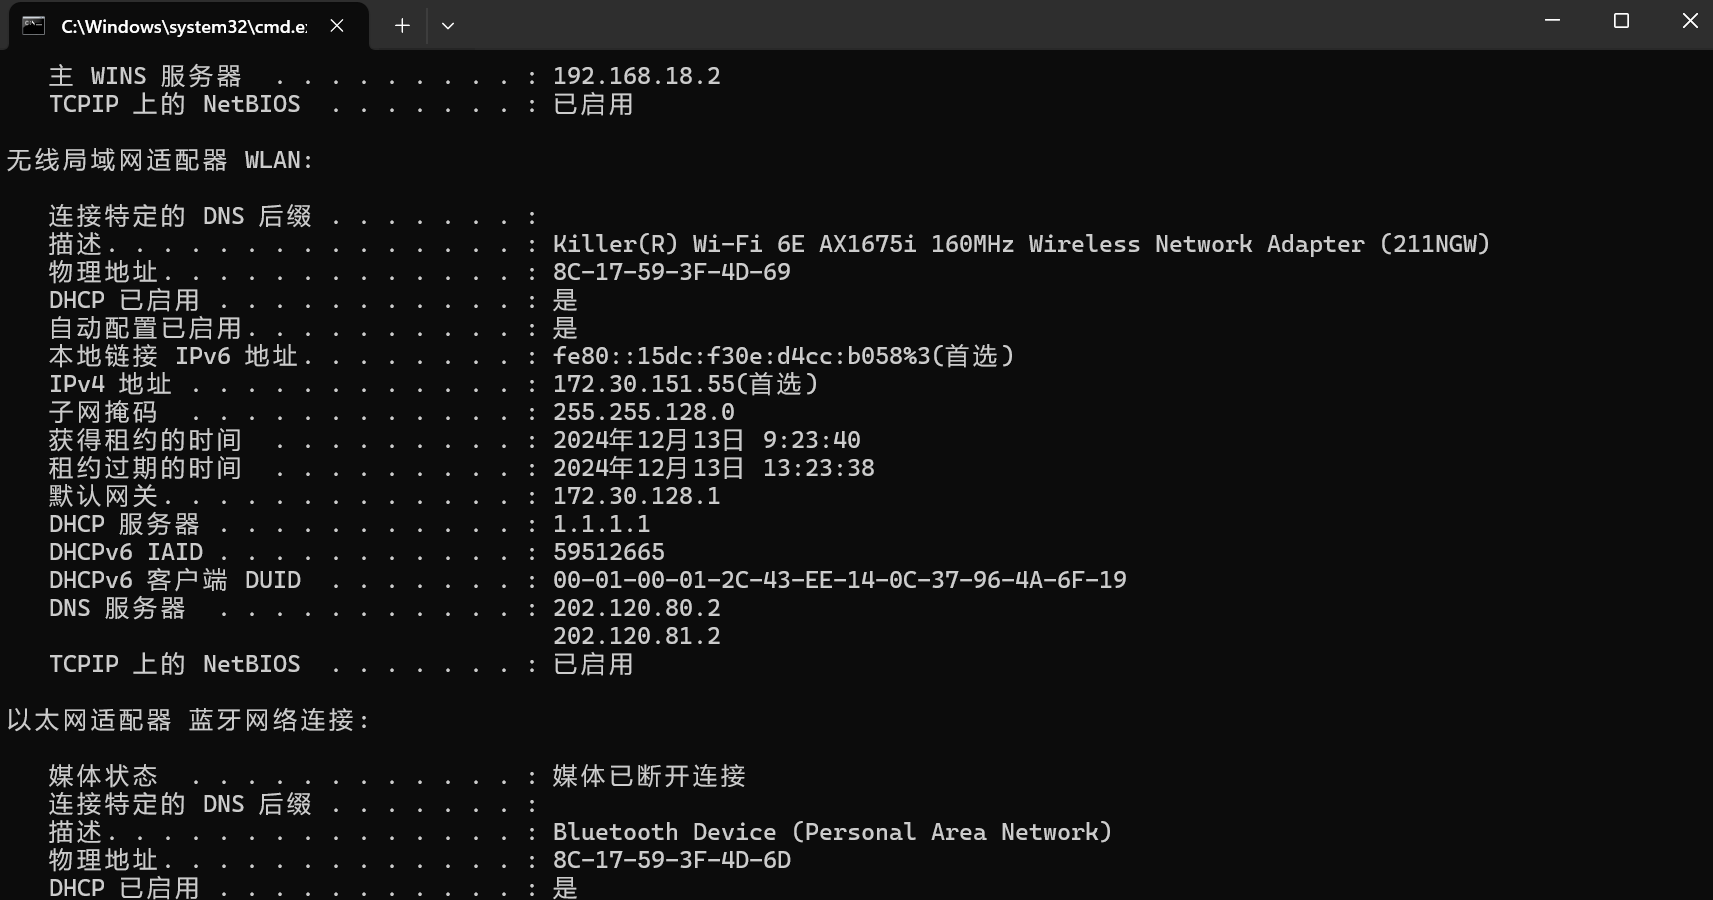
\includegraphics[width=11cm]{images/2.获取本机IP地址和MAC地址.png}
		\caption{获取本机IP地址和MAC地址}
	\end{figure}
	
	可以看到,本机的 \texttt{IP} 地址为 \texttt{172.30.151.55}, \texttt{MAC} 地址为 \texttt{8C-17-59-3F-4D-69}。
	
	回到\texttt{Wireshark},设置捕获过滤器为 \texttt{eth.addr==8C-17-59-3F-4D-69}。
	
	\begin{figure}[H]
		\centering
		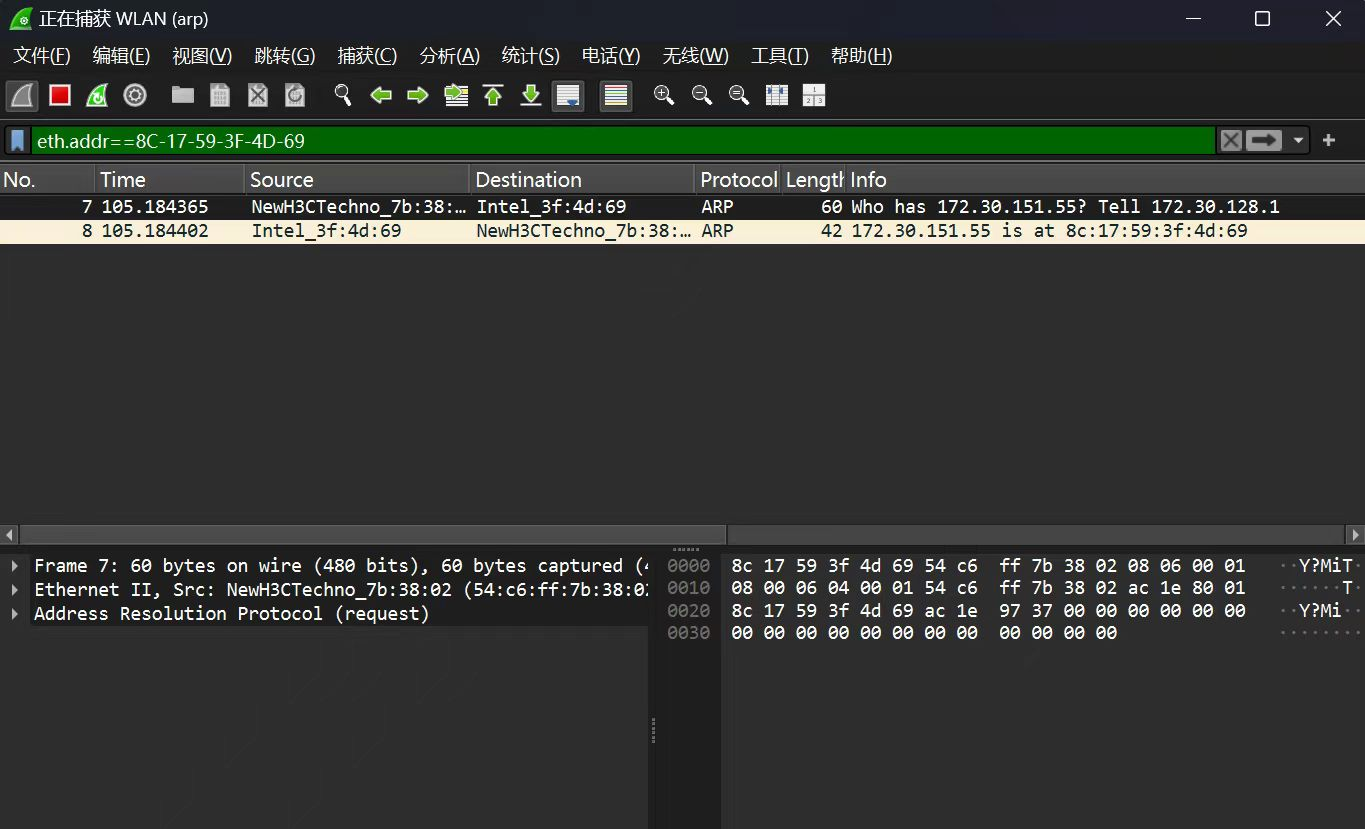
\includegraphics[width=10cm]{images/3.设置捕获过滤器.jpg}
		\caption{设置捕获过滤器}
	\end{figure}
	
	接下来,在管理员模式下,在命令提示符中使用 \texttt{arp -d} 命令清除本机的 \texttt{ARP} 缓存。
	
	\begin{figure}[H]
		\centering
		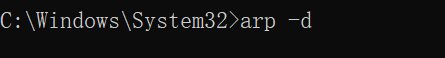
\includegraphics[width=10cm]{images/4.清除本机ARP缓存.png}
		\caption{清除本机ARP缓存}
	\end{figure}
	
	打开 \texttt{Wireshark},停止捕获。捕获结果如下图所示:
	
	\begin{figure}[H]
		\centering
		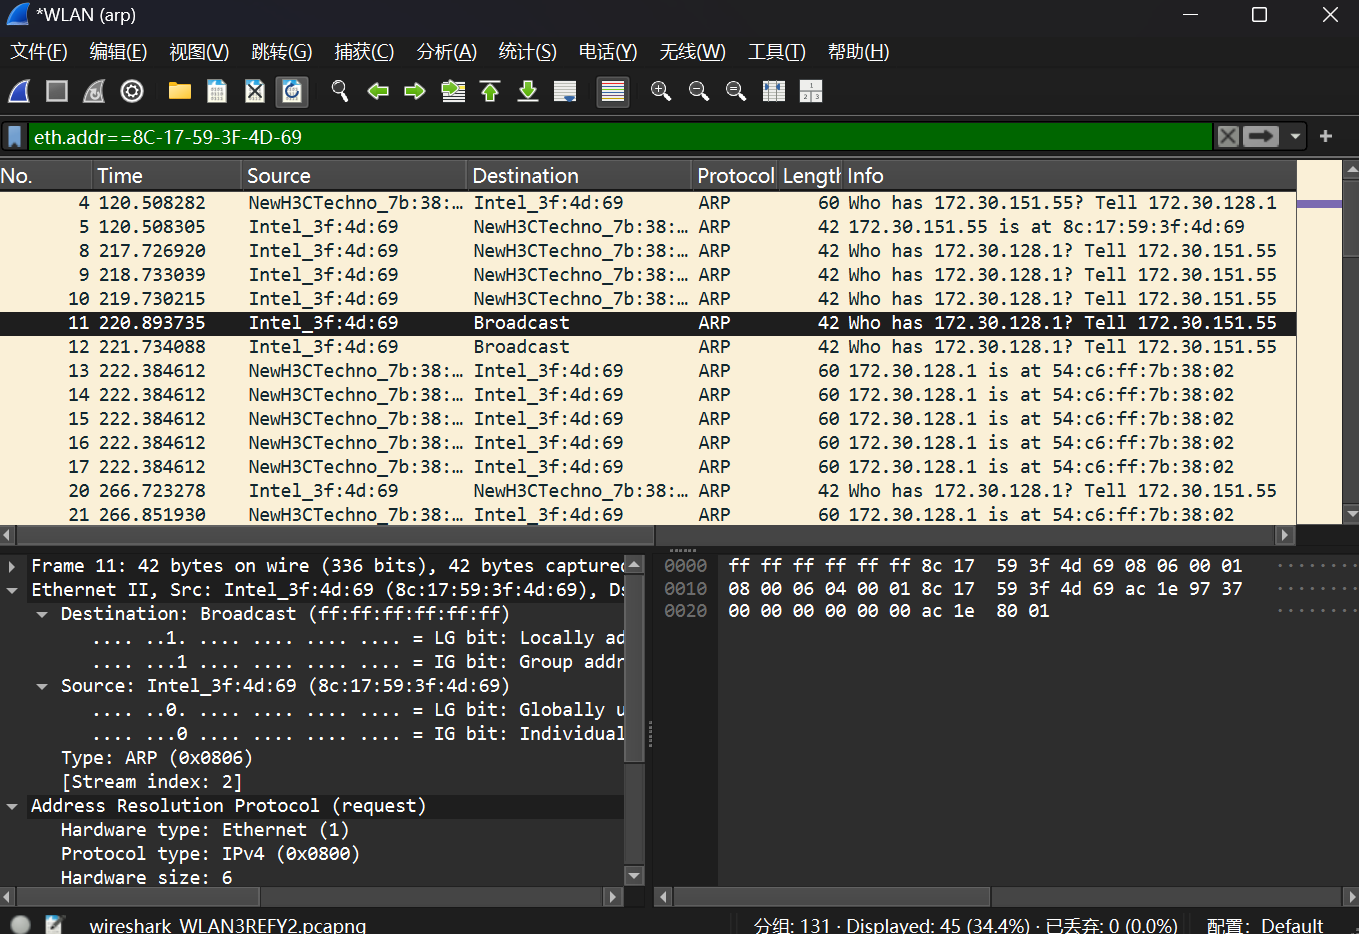
\includegraphics[width=10cm]{images/5.捕获结果.png}
		\caption{捕获结果}
	\end{figure}
	
	\subsection{回答问题}
	
	\begin{enumerate}
		\item Hand in your drawing of the ARP exchange.
		
		选择 \texttt{ARP} 请求数据包,如下图所示:
		
		\begin{figure}[H]
			\centering
			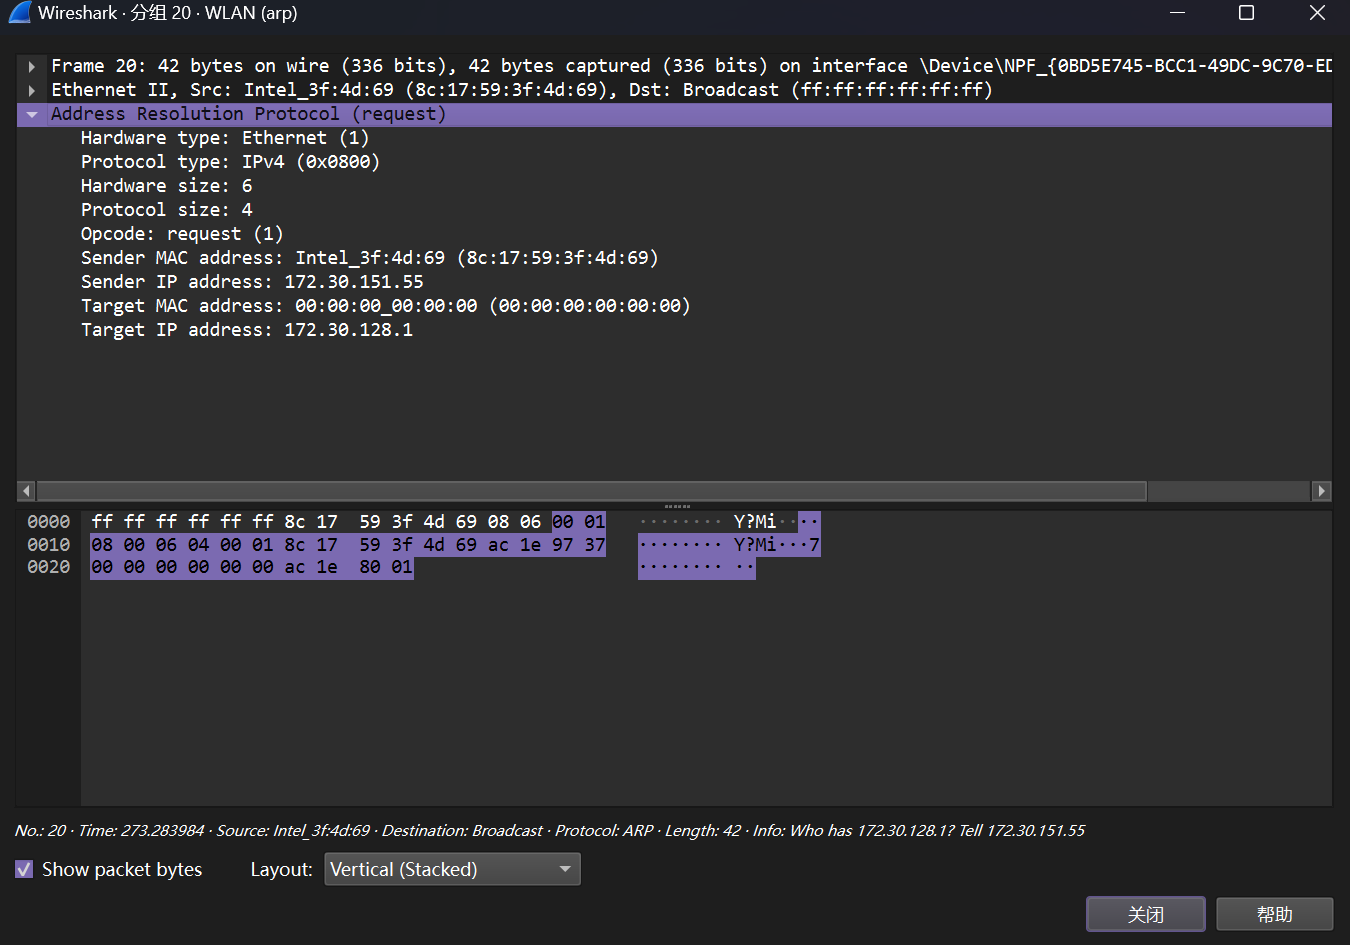
\includegraphics[width=10cm]{images/6.选择ARP请求数据包.png}
			\caption{选择ARP请求数据包}
		\end{figure}
		
		可以看到,它包括了一个长度为 28 字节的 \texttt{ARP} 报头,其中包括了以下字段:
		
		\begin{itemize}[noitemsep]
			\item Hardware type: Ethernet (1),长度为 2 字节
			\item Protocol type: \texttt{IPv4}(0x0800),长度为 2 字节
			\item Hardware size: 6,长度为 1 字节
			\item Protocol size: 4,长度为 1 字节
			\item Opcode: request (1),长度为 2 字节
			\item Sender MAC address: \texttt{8c:17:59:3f:4d:69},长度为 6 字节
			\item Sender IP address: \texttt{172.30.151.55},长度为 4 字节
			\item Target MAC address: \texttt{00:00:00:00:00:00},长度为 6 字节
			\item Target IP address: \texttt{172.30.128.1},长度为 4 字节
		\end{itemize}
		
		画出 \texttt{ARP} 请求数据包,如下图所示:
		
		\begin{figure}[H]
			\centering
			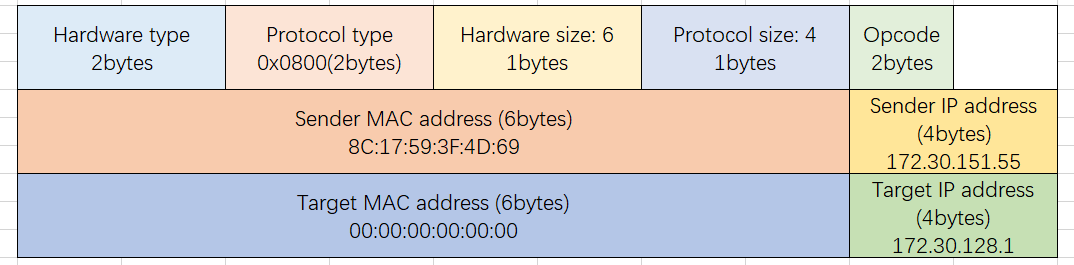
\includegraphics[width=11cm]{images/7.ARP请求数据包.png}
			\caption{ARP请求数据包}
		\end{figure}
		
		选择一个 \texttt{ARP} 应答数据包,如下图所示:
		
		\begin{figure}[H]
			\centering
			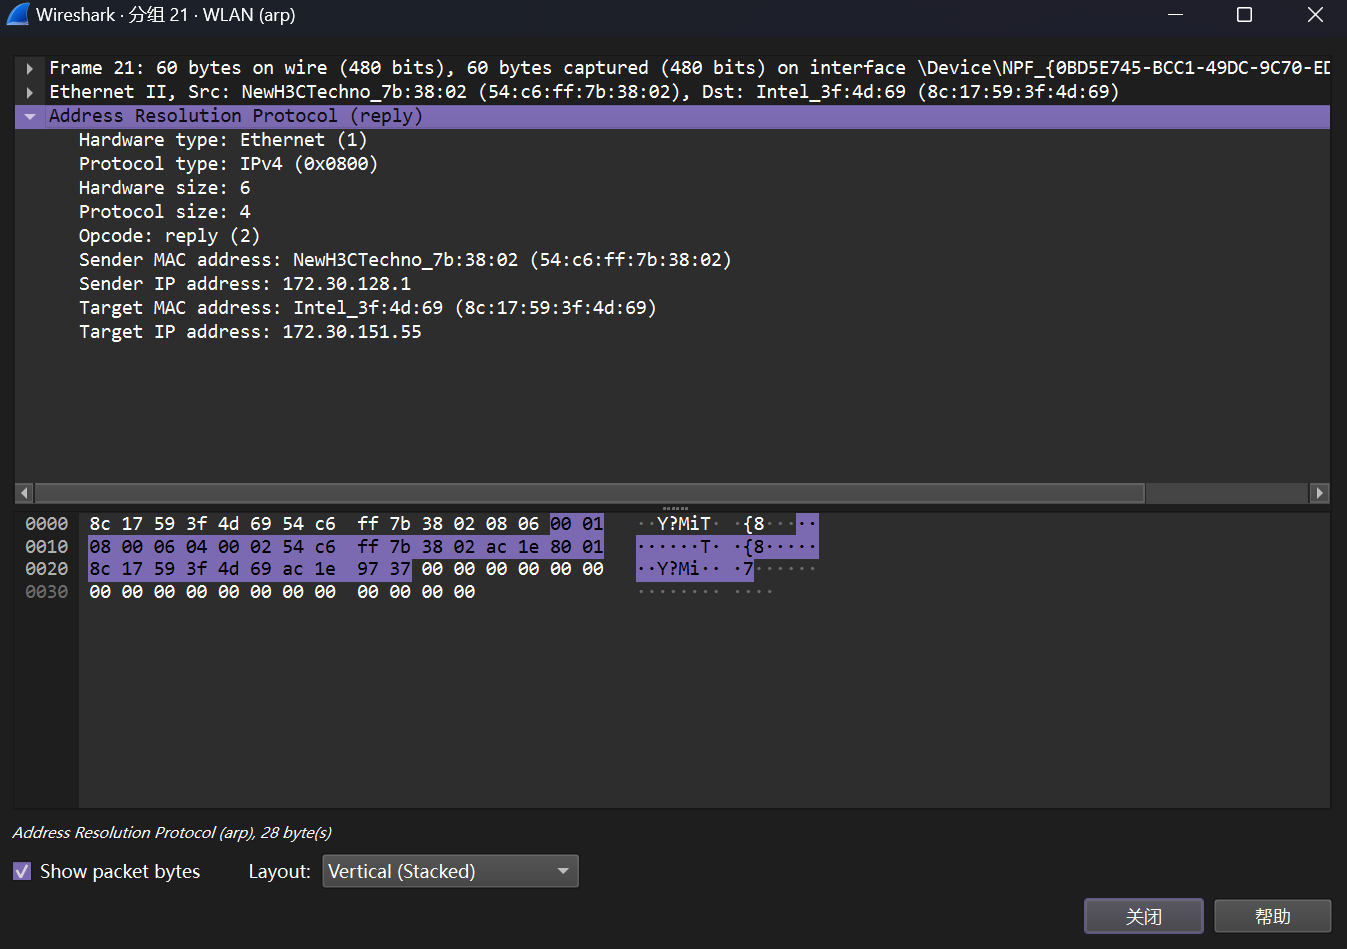
\includegraphics[width=11cm]{images/8.选择ARP应答数据包.png}
			\caption{选择ARP应答数据包}
		\end{figure}
		
		画出 \texttt{ARP} 应答数据包,如下图所示:
		
		\begin{figure}[H]
			\centering
			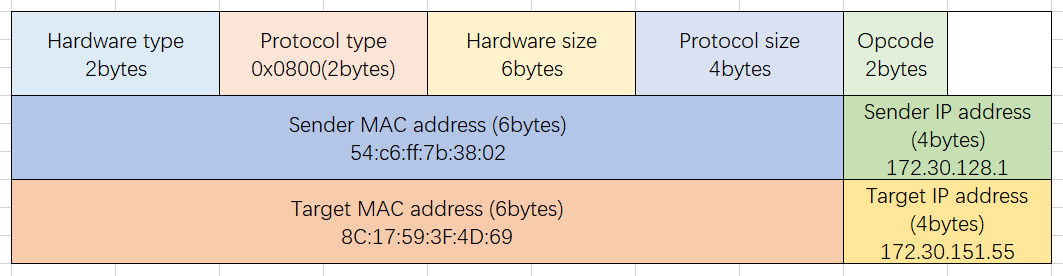
\includegraphics[width=11cm]{images/9.ARP应答数据包.png}
			\caption{ARP应答数据包}
		\end{figure}
		
		\item What opcode is used to indicate a request? What about a reply?
		
		\texttt{ARP} 报头中的 \texttt{Opcode} 字段用于表示 \texttt{ARP} 请求或应答,其中 \texttt{Opcode} 值为 1 表示请求,值为 2 表示应答。
		
		
		\item How large is the ARP header for a request? What about for a reply?
		
		二者长度均为 28 字节。
		
		\item What value is carried on a request for the unknown target MAC address?
		
		对未知目标的 \texttt{MAC} 地址的请求是 \texttt{00:00:00:00:00:00}。
		
		\item What Ethernet Type value which indicates that ARP is the higher layer protocol?
		
		以太网类型值为 \texttt{0x0806} 表明 \texttt{ARP} 是更高一层的协议。
		
		\begin{figure}[H]
			\centering
			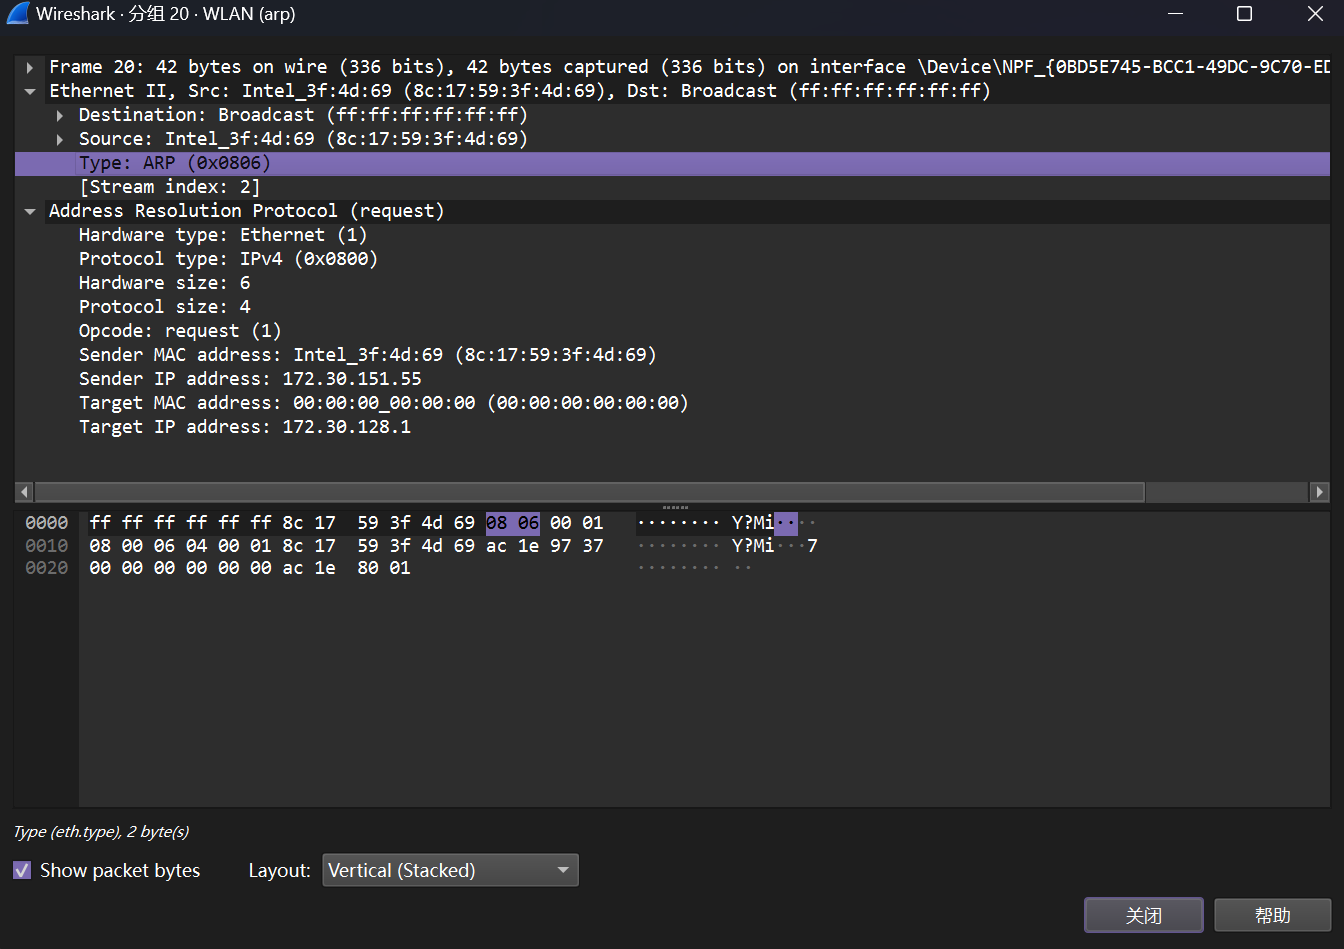
\includegraphics[width=11cm]{images/10.ARP的类型值为0x0806.png}
			\caption{ARP的类型值为0x0806}
		\end{figure}
		
		\item Is the ARP reply broadcast (like the ARP request) or not?
		
		在以太网层可以观察到,\texttt{ARP} 应答是单播。
		
		\begin{figure}[H]
			\centering
			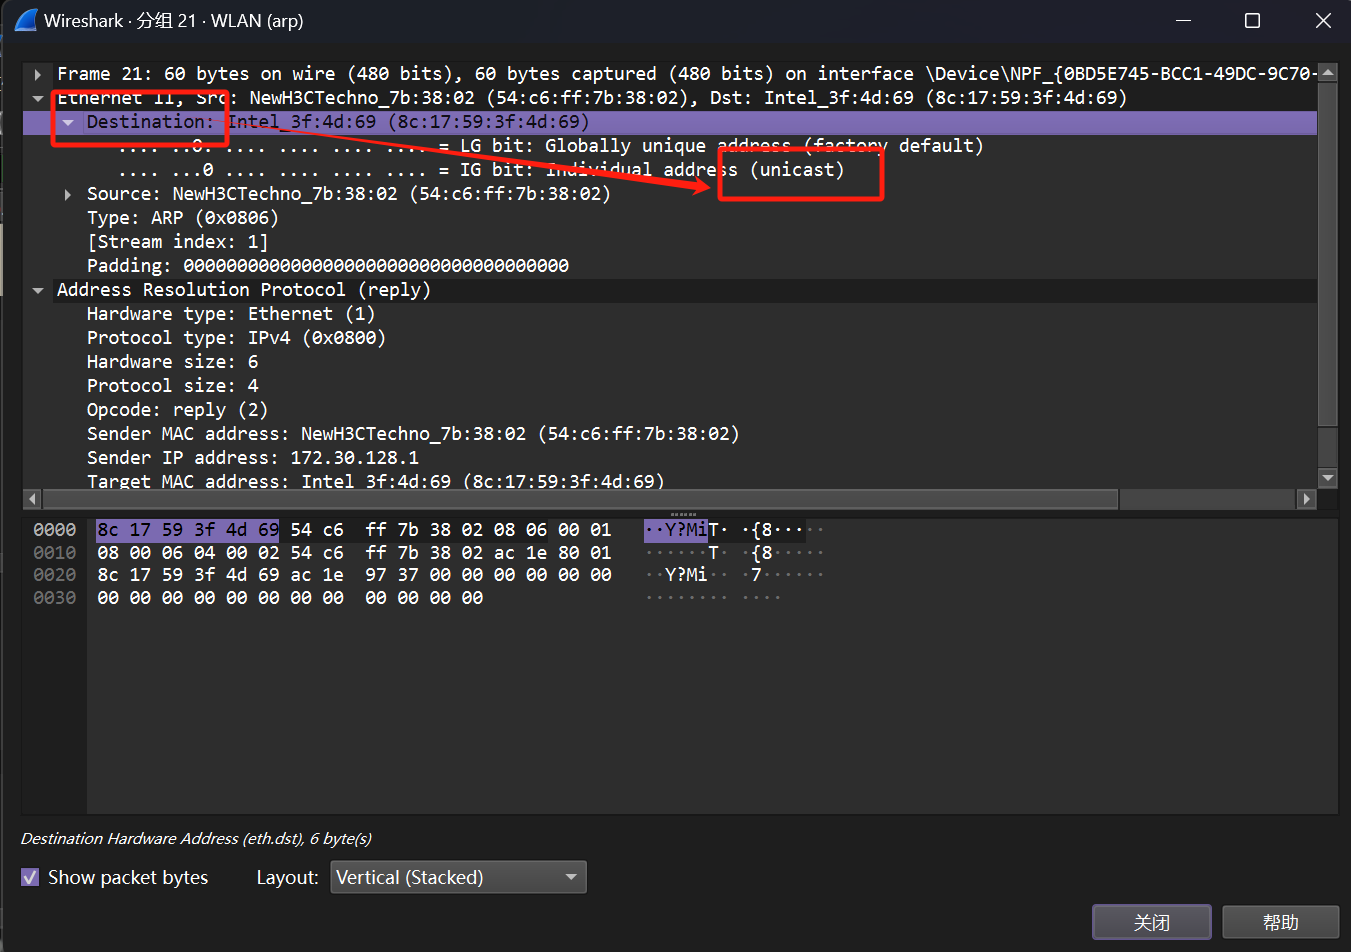
\includegraphics[width=11cm]{images/11.ARP应答是单播.png}
			\caption{ARP应答是单播}
		\end{figure}
		
	\end{enumerate}
	
	\subsection{问题讨论}
	
	We encourage you to explore ARP on your own once you have completed this lab. One suggestion is to look at other ARP packets that may have been recorded in your trace; we only examined an ARP request by your computer and the ARP reply from the default gateway. 
	
	\begin{enumerate}
		
		\item ARP requests broadcast by other computers. The other computers on the local network are also using ARP. Since requests are broadcast, your computer will receive their requests. 
		
		清除过滤器后,可以观察到其他计算机发送的 \texttt{ARP} 请求。
		
		\begin{figure}[H]
			\centering
			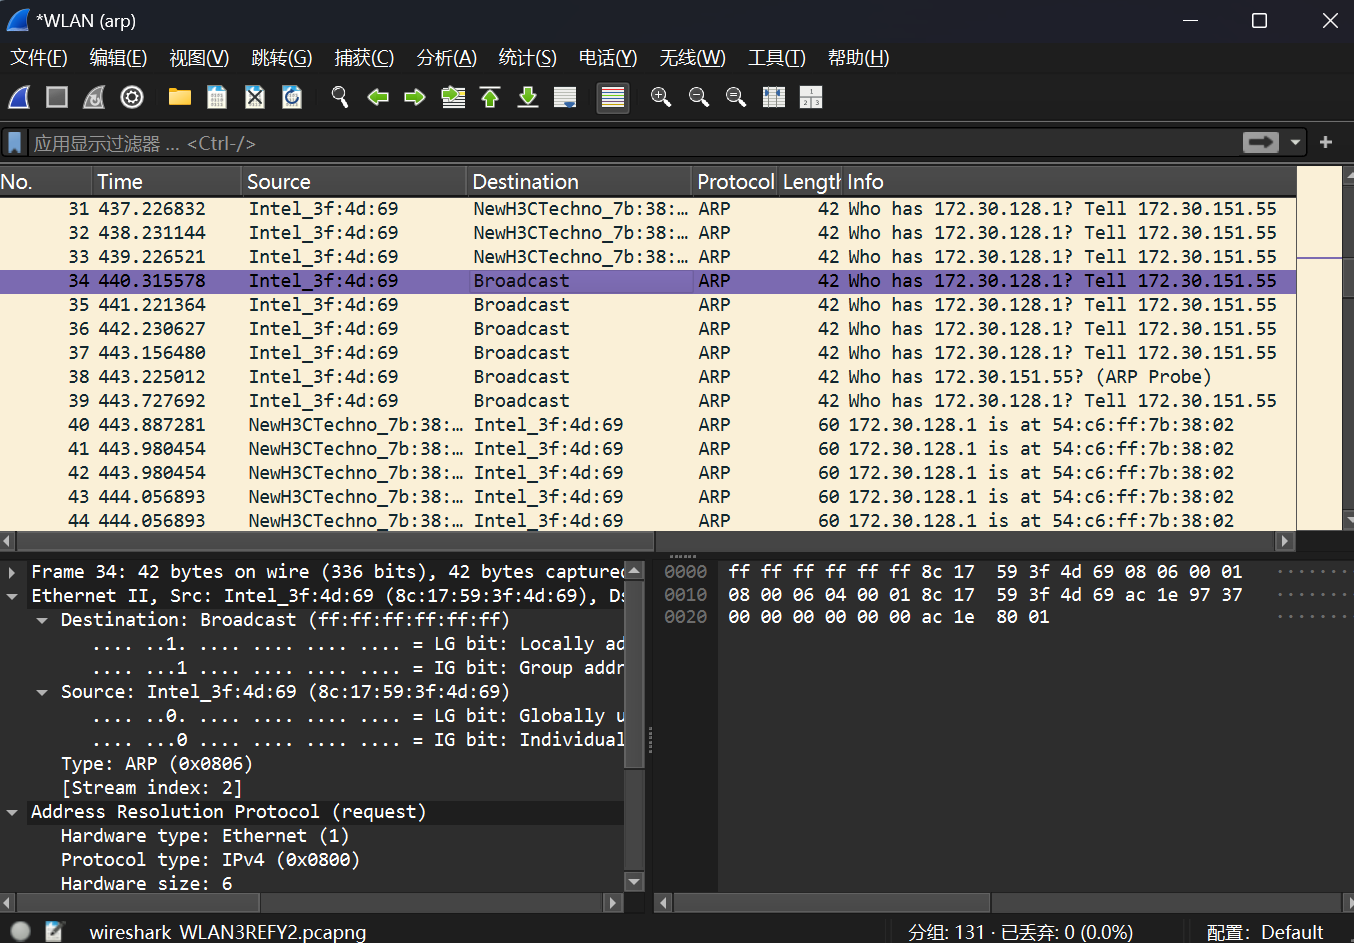
\includegraphics[width=11cm]{images/12.其他计算机发送的ARP请求.png}
			\caption{其他计算机发送的ARP请求}
		\end{figure}
		
		\item ARP replies sent by your computer. If another computer happens to ARP for the IP address of your computer, then your computer will send an ARP reply to tell it the answer. 
		
		可以在另一台计算机上使用 \texttt{arp -d 172.30.151.55} 命令清除 \texttt{ARP} 缓存,然后使用 \texttt{ping 172.30.151.55} 命令向本机发送 \texttt{ICMP} 请求,此时也会发起一个 \texttt{ARP} 请求,本机随后会发送 \texttt{ARP} 应答,如下图所示:
		
		\begin{figure}[H]
			\centering
			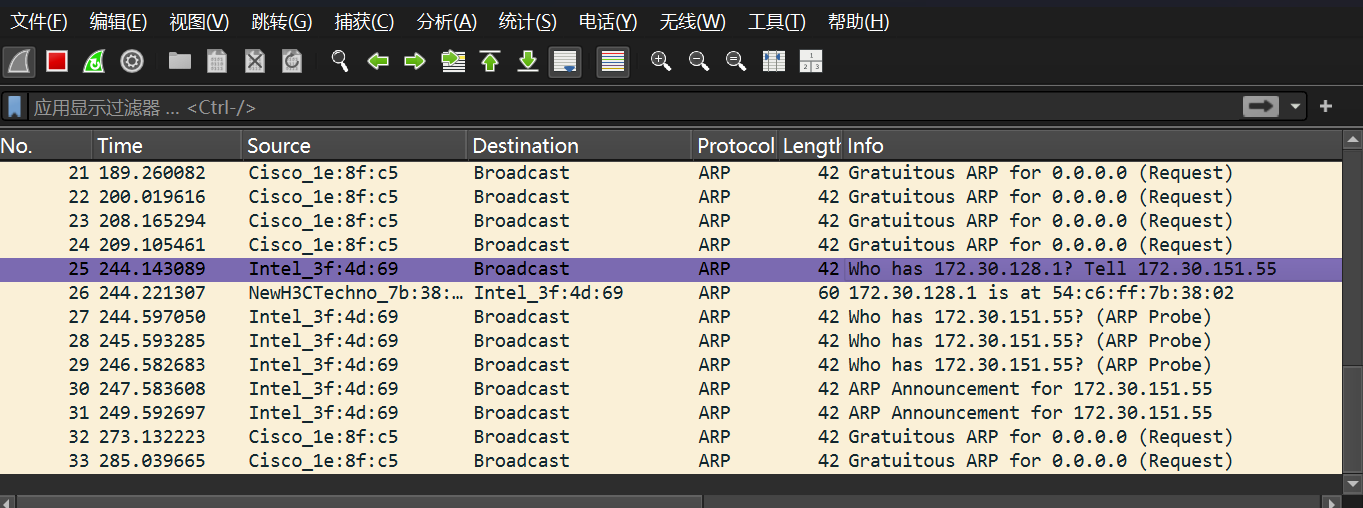
\includegraphics[width=11cm]{images/13.本机发送了ARP应答.png}
			\caption{本机发送了ARP应答}
		\end{figure}
		
		\item Gratuitous ARPs in which your computer sends a request or reply about itself. This is helpful when a computer or link comes up to make sure that no-one else is using the same IP address. Gratuitous ARPs have the same sender and target IP address, and they have an Info field in Wireshark that identified them as gratuitous.
		
		可以在捕获列表中看到 \texttt{gratuitous ARP} 数据包。
		
		\begin{figure}[H]
			\centering
			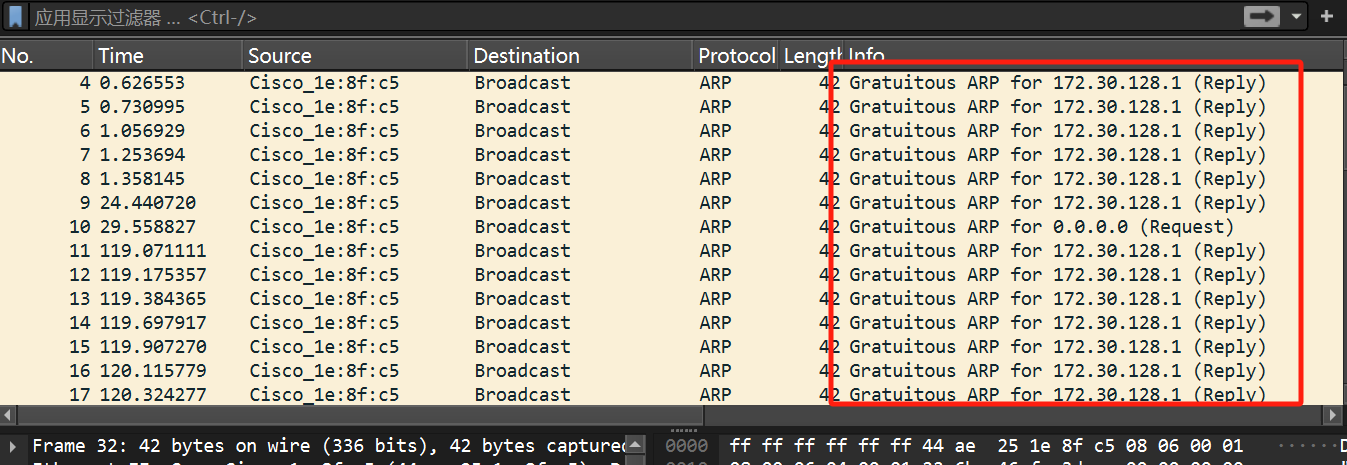
\includegraphics[width=11cm]{images/14.捕获到的gratuitous ARP 数据包.png}
			\caption{捕获到的gratuitous ARP 数据包}
		\end{figure}
		
		\item Other ARP requests sent by your computer and the corresponding ARP reply. Your computer may need to ARP for other hosts besides the default gateway after you flush its ARP cache. 
		
		清除 \texttt{ARP} 缓存后,可以观察到相关请求。
		
		\begin{figure}[H]
			\centering
			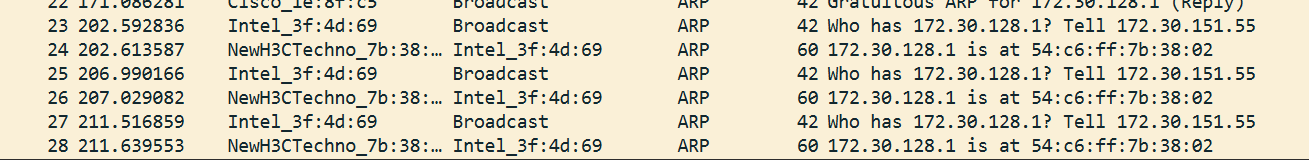
\includegraphics[width=11cm]{images/15.相关请求.png}
			\caption{相关请求}
		\end{figure}
	\end{enumerate}
	
	\section{实验结果总结}
	
	本次实验利用 \texttt{Wireshark} 捕获了 \texttt{ARP} 数据包,并通过对其进行详细分析,深入理解了 \texttt{ARP} 数据包的结构及其各字段的含义,从而进一步加深了对 \texttt{ARP} 协议的认识。
	
	
	\section{附录}
	
	无
	
\end{document}